\chapter{Introduction}

\section{Motivation}

The expression Internet of Things is relatively new, was coined between 1997 and 2000 and consists of devices that sense or actuate in a real environment (\cite{minerva2015towards}). The number of IoT devices has already overcame the living humans on Earth and, by 2020, is estimated to exist about 20 billion of IoT devices connected to the internet \citep{iotmarket}. It is very common that these devices have a companion app, cloud or mobile based which are used to control and monitor the IoT devices.

This growing popularity come along with major security and privacy issues, hackers are exploiting Android apps to leak user private information or hijacking the IoT device to use in other attacks, such as DDoS \citep{ycraig}. The information leak is very concerning from a privacy point of view, as a vast majority of user sensitive information is stored in smartphones, GPS location, text messages, photos and even bank data can be stolen if exists an issue in IoT companion apps.

IoT applications consists in a device that can sense and actuate in the real environment which is controlled and monitored using mobile apps or a web server to serve for any kind of purpose, from medical monitoring to smart wearable devices. Depending of the application the devices are designed to last for years with low or no need of maintenance or be portable. To ensure that these devices are hardware constrained, lacking computational power to ensure a longer battery life \citep{raj2017internet}. This leads to some issues: the needing of newer lightweight security protocols to fit the hardware constrains as \cite{zhang2014iot} points and a reduced set of communications protocols and interfaces to keep low power consumption.

The lack of communications protocols forced the industry to create other devices to act as an IoT hub, if the IoT does not have an independent connection to the internet, hub architectures are common if the device have simpler and short communication protocols, like Bluetooth, RFID, ZigBee and NFC \cite{al2017internet}. The hub concentrate the communications between the devices and the companion app, this app is a mobile or cloud application that provides monitoring and control for the IoT devices. The real IoT communication architecture is very diverse but a device have few options, it can only send information through the hub to the cloud, to a smartphone, directly to the cloud or have these three combined using a mixed architecture.

In Figure \ref{fig:arch-direct} we can observe how the IoT device communicate directly to user devices, the smart devices are represented by a smart bulb and the user devices by a smartphone and a desktop computer. The full arrows express that that the link must exist to have a connection. In Figure \ref{fig:arch-hub}, we have a intermediate device that makes the connection between the device and the user, the hub can aggregate as many IoT devices as intended. The cloud architecture Figure \ref{fig:arch-cloud} consists in a device that is connected to the internet using a router, which sends and receives user actions using the cloud as intermediary. The mixed architecture, Figure \ref{fig:arch-mixed}, can have all the previous kind of connections, the user has freedom to send information directly to the device, or use a hub to control the devices with only one application or send remote requests using any cloud provider.

\begin{figure}[ht] 
    \begin{minipage}[b]{0.5\linewidth}
        \centering
        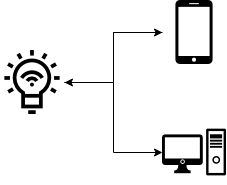
\includegraphics[width=0.6\linewidth]{images/iot-architectures/direct.png}
        \caption{Direct architecture}\label{fig:arch-direct}
        \vspace{4ex}
    \end{minipage}%%
    \begin{minipage}[b]{0.5\linewidth}
        \centering
        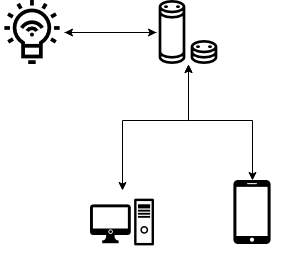
\includegraphics[width=0.6\linewidth]{images/iot-architectures/hub.png}
        \caption{Hub architecture}\label{fig:arch-hub}
        \vspace{4ex}
    \end{minipage} 
    \begin{minipage}[b]{0.5\linewidth}
        \centering
        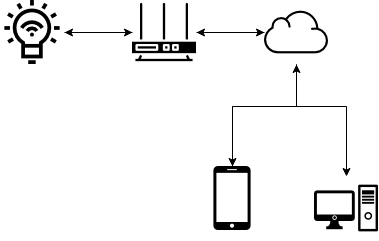
\includegraphics[width=0.8\linewidth]{images/iot-architectures/cloud.png}
        \caption{Cloud based architecture}\label{fig:arch-cloud}
        \vspace{4ex}
    \end{minipage}%% 
    \begin{minipage}[b]{0.5\linewidth}
        \centering
        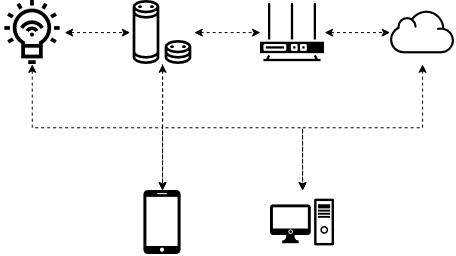
\includegraphics[width=1\linewidth]{images/iot-architectures/mixed.png}
        \caption{Mixed architecture}\label{fig:arch-mixed}
        \vspace{4ex}
    \end{minipage} 
\end{figure}

With the increasing popularity of IoT, attackers are exploiting weakness in the architecture, the device itself and the smartphones that hosts the application. Exists many known attacks, from leaking user data as described by \cite{ycraig} to hijacking the device to use in other attacks such as DDoS using botnets \citep{kolias2017ddos}. The information leaking is a major concern from a privacy point of view, this kind of attack can leak any kind of user sensitive data being sent to malicious hosts or unaware to a cloud server. 

Sensitive data is any data that can be used to identify the user or any private user information, such as photos, International Mobile Equipment Identity (IMEI), biometric data, GPS localization, bank information and private messages. Non-sensitive data is any dynamic information that do not identify the user, often, this kind of information if public or shared, such as application source code.

Every program computes on either sensitive data or non-sensitive data, and this data follows a specific flow, first it is acquired from data sources and sent to data sinks \citep{mccabe2003network}. Data sources, in the context of mobile and IoT devices, are defined as method calls that read data from shared resources such as phone calls, screenshots, sensor polling data from ambient, device identification numbers \citep{rasthofer2014machine}. Data sinks are methods calls that have at least one argument, this argument is non-constant data from the source code \citep{rasthofer2014machine}. The data sink can be an interface to the user or system API for communication to other devices or store data \citep{viet2010specifying}.

To address the data privacy issue, mobile operating systems such as Android and IOs have a permission based system intended to control which sensitive information the application have access, like contact numbers, photos, videos and data from camera and microphone. These permissions are granted by the user at the installation or during the application usage (\cite{androidpermissions}). An issue existing in the permission system is called superprivileges, where the apps asks for unnecessary permissions, caused by developers that misunderstanding the API (\cite{felt2011android}). There is a methodology that help the developers to have a broader knowledge of the permissions in Android that has been proposed by \cite{barrera2010methodology}.

Another issue created when using the permission system is the abuse of privilege given by the user to an app, or even, the application can intentionally send information to a malicious host. As \cite{jiang2012dissecting} reports, there are malwares that are capable to steal sensitive information from the user, like SMS. To solve unwanted sensitive information flow inside Android applications, \cite{arzt2014flowdroid}, \cite{wei2014amandroid} and \cite{gordon2015information} developed static and dynamic ways to enforce that this kind of information does not leak to unwanted sink methods. The dynamic way to enforce information flow is called Dyanmic Flow Enforcement and statically is called Static Flow Enforcement. These methods are going to be presented in a deeper fashion in Chapter \ref{chapter:background}.


\section{Objective}\label{section:background}

This work has two main objectives: generate a public database containing methods from Android APIs and evaluate the performance of the most used classification algorithms on this database. The methods should be classified into source or sink, or neithernor.

The motivation behind the database creation comes when \cite{rasthofer2014machine} developed the initial classification work. Their objective were create a machine-learning solution to identify sources and sink methods from the code of any Android API. So, every time that you wanted to test other classification algorithms, you had  to extract the methods and features at every execution. Then, create a public database extract knowledge and  develop better solutions to this problem is very likely.

The objective of evaluate different classification algorithms comes as \cite{rasthofer2014machine} shows results  for only three classification algorithms, SVM, Decision Tree and Naive Bayes. From that, emerged the question if other classification algorithms have better results in this database. So, the second objective is to evaluate the most used classifiers in the literature, SVM, Naive Bayes, Decision Trees, MLP, KNN, including ensemble classifications methods.


\section{Work Structure}\label{section:structure}

This work is divided as follows: Chapter \ref{chapter:background} is a short introduction about Static and Dynamic Analysis, followed by a explanation about Flow Enforcement techniques, which is important to understand what issues these methods addresses and what are the limitations. In Chapter \ref{chapter:architecture} we introduce the methodology used in this work and the training and test architectures used by the machine learning methods. \ref{chapter:results} we show the results archived, the dataset created and the scores of each classifier used in this work and we report our conclusions in \ref{chapter:conclusion}.
